%!TEX root = ../Peerbox.tex



%  It also helps to avoid unwanted message transmission and prevents clogging of networks and conserves bandwidth.
% % The IP address 224.0.0.0 through 239.255.255.255 are reserved for multicasts. The user needs to set some properties such as Path, Multicast address, Multicast port, Server Port and the name of the computer.
% Also, as messages are UDP, there is no need for connection set-up or teardown. The Peerbox system can be used across LAN.

arch overview. 

layers

communication

communication between peers via multicast 
file transmission via direct peer-to-peer




\subsection{Middleware}

requires coordination and 
agreement
agree on the set of messages received or on delivery 
ordering

FIFO-ordering
why we do not want Total ordering


properties


however ip multicast is per se unreliable, early test have shown a miss rate of 20\%

over udp datagram

negative acknowledgements

reliable multicast

additional checksum to verify payload

\subsubsection{Messages}

%figure message package

command can be either Message (1), ACK(2) or NACK(4). 
Acks are not used in this implementation in order to reduce traffic on the channel 

the size of the payload is dynamic though it is not allowed to be larger than the maximum message size, which is in our case preset to $2^15$. A fixed message size is important in order to determine the number of sizes from incoming messages. 


However, if the logic needs to send a lot of data, it can be split onto multiple messages (due to the reliable multicast it is guaranteed that all messages will eventually arrive and are consumed in order).


\subsubsection{Delivering Messages form Group}


\begin{figure}[htbp]
    \centering
        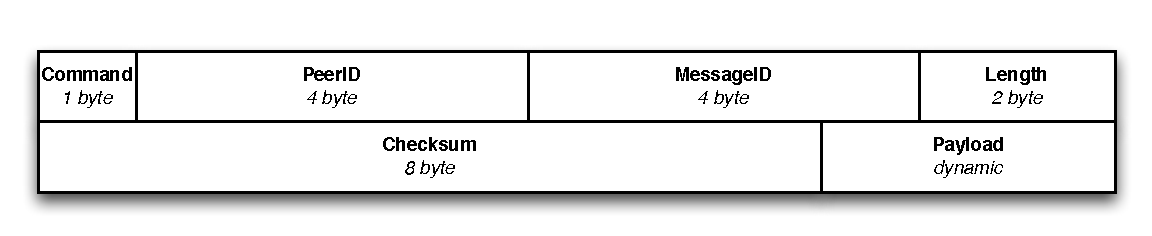
\includegraphics[width=.9\textwidth]{figures/message.pdf}
    \caption{Structure of a message}
    \label{fig:figures_announcement}
\end{figure}

use of resources  is indicated by a dashed line 
processes are divided by swim-lanes (dotted vertical lines)

\begin{figure}[htbp]
    \centering
        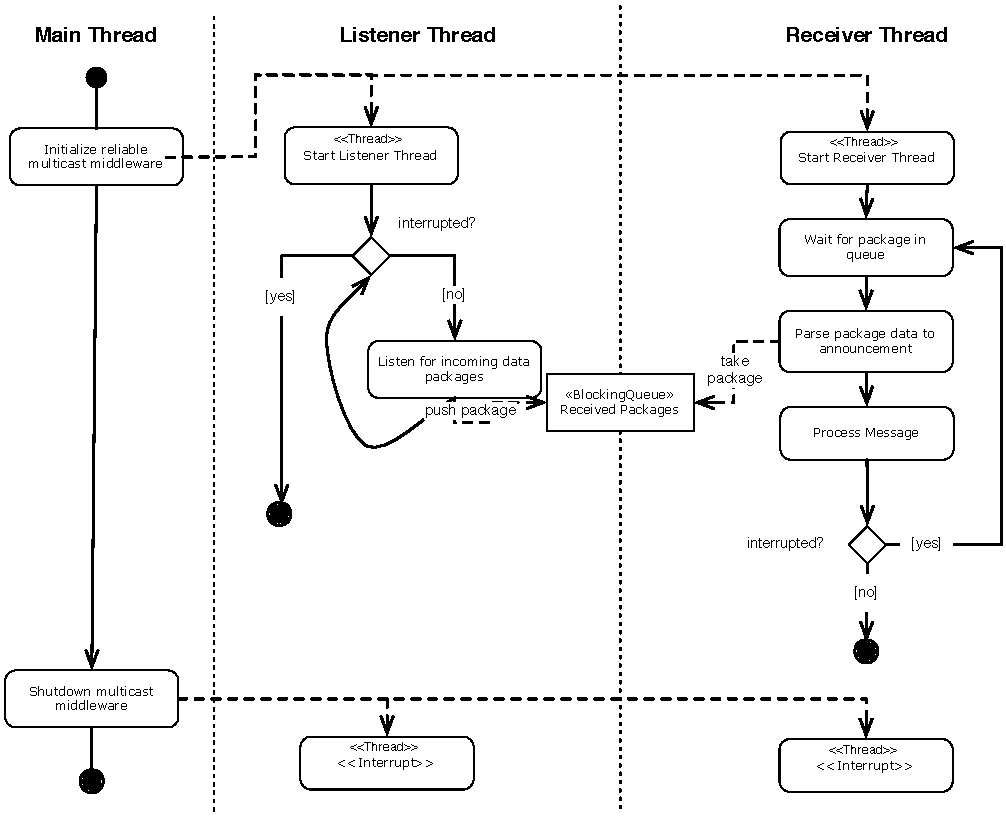
\includegraphics[height=4.5in]{figures/receivePackets.pdf}
    \caption{Listen for incoming multicast messages}
    \label{fig:figures_processReceivePackage}
\end{figure}

\begin{figure}[htbp]
    \centering
        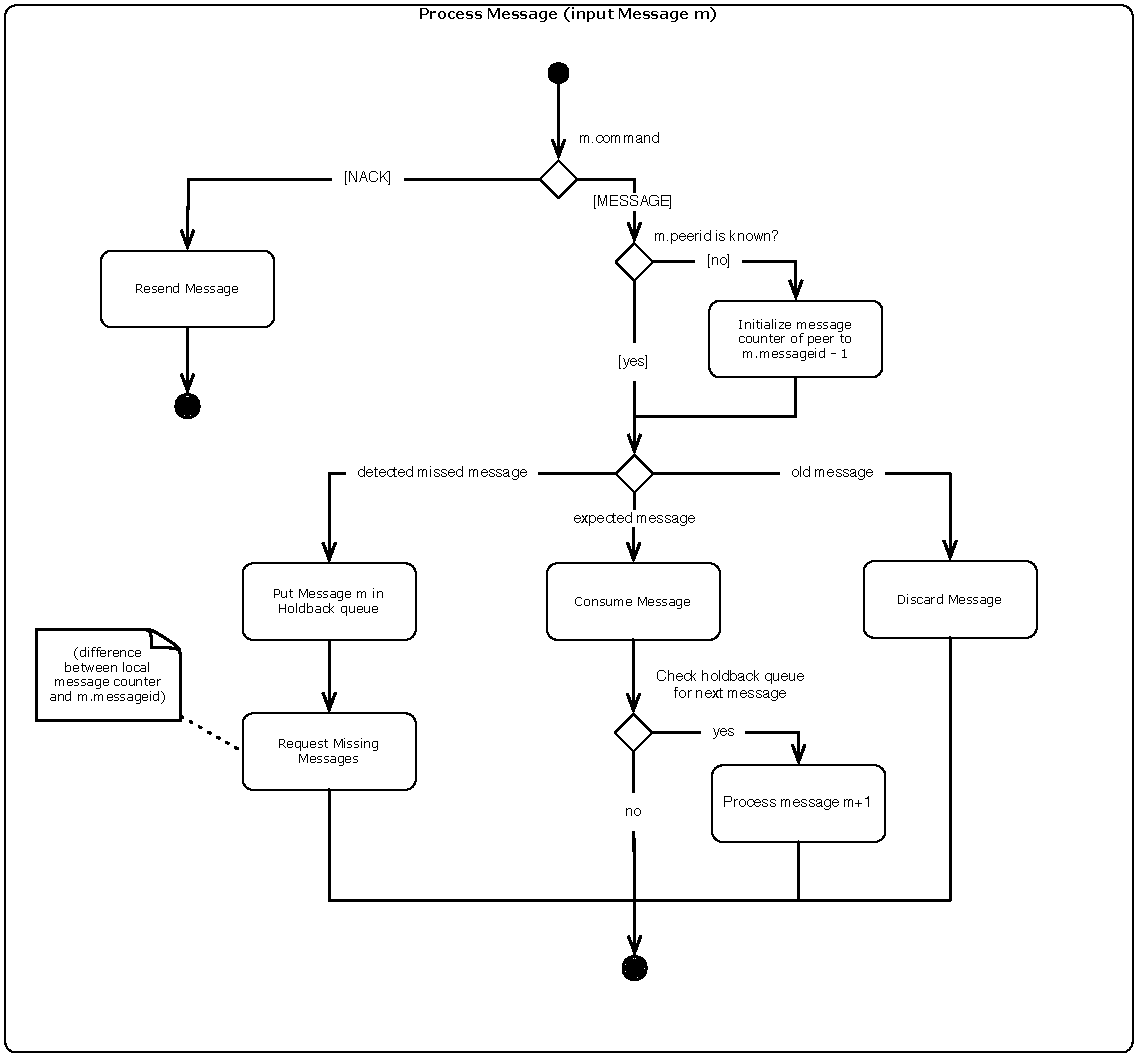
\includegraphics[height=4.5in]{figures/processMessages.pdf}
    \caption{Process incoming multicast messages}
    \label{fig:figures_processMessages}
\end{figure}

\subsubsection{Sending Messages to Group}

\begin{figure}[htbp]
    \centering
        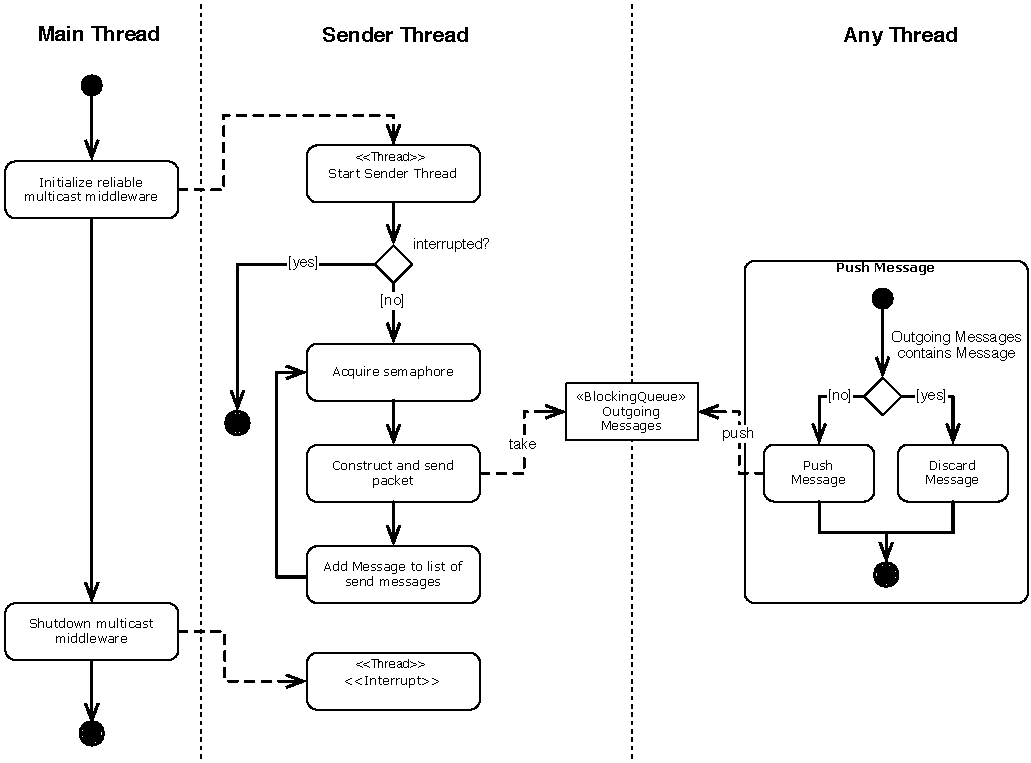
\includegraphics[height=4in]{figures/sendMessage.pdf}
    \caption{Send a multicast message}
    \label{fig:figures_processMessages}
\end{figure}

\subsubsection{Optimizations}

limit bandwidth 
    - should be made dynamic
    
queue optimizations (discard duplicate)

\subsection{Logic}

    
    \subsubsection{Messages}
    serialized dictionary
    dynamic structure realized by a serialized key-value store. 
    this allows to easily extend the protocol


    \subsubsection{Message handling}
    Strategy pattern, depending on the Key.Command the appropriate handler will be chosen.
    
    \subsubsection{VirtualFileSystem}
    
    observe folder changes
    
    associate files with peers
    
    limitation: no real fs, hence it is possible to invalidate the state of the vfs by modifying the folder when the application is not running. 
    
    \subsubsection{Requesting a file}
    
    direct communication, multicasting files might be inappropriate
    
    \subsubsection{Fault-tolerance Hearbeat}
    toughest challenge in async network, what happens when peer leaves without notice (e.g. crashed). On the one hand, it is not possible to distingush between a crash or a slow peer and  on the other hand there is no automatic mechanism that detects if a peer left a multicast group.
    
    Therefore we implement a (Heartbeat), we favored a heartbeat over a ping tactic because we do not need to elect a leader for that. 
    every peer send a heartbeat every x second with its vector clock (showing its internal message state), if a peer 
    
    this might cause that a peer is temporarily not available also he is functioning properly.
    

    
    
    

\subsection{Interface}